\documentclass[sigconf]{acmart}
%%
%% \BibTeX command to typeset BibTeX logo in the docs
\AtBeginDocument{%
  \providecommand\BibTeX{{%
    Bib\TeX}}}


%% start of the body of the document source.
\begin{document}
\title{Retinal Classification in the Transformer Age}

%%
%% The "author" command and its associated commands are used to define
%% the authors and their affiliations.
%% Of note is the shared affiliation of the first two authors, and the
%% "authornote" and "authornotemark" commands
%% used to denote shared contribution to the research.
\author{Derek Burrola}
\email{djb4994@utexas.edu}
\affiliation{%
  \institution{University of Texas at Austin}
  \city{Austin}
  \state{Texas}
  \country{USA}
}

%%
%% By default, the full list of authors will be used in the page
%% headers. Often, this list is too long, and will overlap
%% other information printed in the page headers. This command allows
%% the author to define a more concise list
%% of authors' names for this purpose.
\renewcommand{\shortauthors}{Burrola.}

%%
%% The abstract is a short summary of the work to be presented in the
%% article.
\begin{abstract}
  Early detection of eye diseases is critical but often limited due to the shortage of ophthalmologists and the high cost of screenings. This study explores the application of Vision Transformer (ViTs) as a preliminary classification of human retinal images. This research builds on previous studies that used convolutional neural networks (CNNs). Through transfer learning from pre-trained ViT models trained on ImageNet-21k, the model is fine-tuned on public datasets to show improvements in precision, recall, and overall accuracy through the use of the ViT architecture reaching accuracies of 94.98\%. The study briefly explores the gained benefits of using ViT over CNNs including attention mechanism and how they can be applied to images to further facilitate the work of ophthalmologists.
\end{abstract}

%%
%% Keywords. The author(s) should pick words that accurately describe
%% the work being presented. Separate the keywords with commas.
\keywords{ViT, retinal, image classification, fundus, vision transformer, medical, AI, medical image classification, eye classification, disease, retinal disease, retinal disease image classification}

%% A "teaser" image appears between the author and affiliation
%% information and the body of the document, and typically spans the
%% page.
\begin{teaserfigure}
  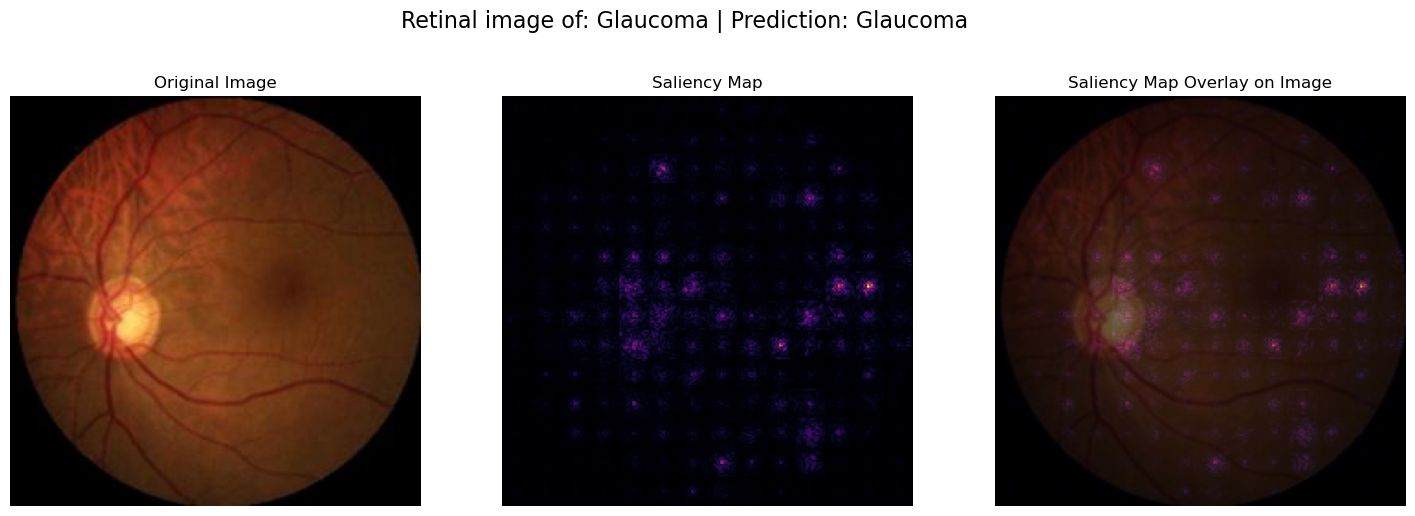
\includegraphics[width=\textwidth]{samples/resources/saliency maps/retinal_glaucoma.png}
  \caption{Retinal Image with Salience Map}
  \Description{3 Images of an eye, a saliency map, and both together}
  \label{fig:teaser}
\end{teaserfigure}

\received{28 April 2025}

%%
%% This command processes the author and affiliation and title
%% information and builds the first part of the formatted document.
\maketitle

\section{Introduction}
Eye-related diseases globally account for millions of affected patients and their treatment exceeds. \$400 billion in the United States alone \cite{Deangelis}. Many of these diseases are either preventable if detected early and can be detected through relatively inexpensive methods such as eye screenings \cite{Forouhi}  While these diseases are easy to detect, and most are simple to treat and even prevent if detected early, the amount of well-trained ophthalmologists is experiencing shortages and the cost for these screenings is become too expensive for most people to consider \cite{Cherlaramani}. In comparison, a computer trained eye screening model can be created at a relatively inexpensive price. This research paper builds on the learned knowledge from Burrola \cite{Burrola}, where pre-trained CNNS were used to classify fundus images.

Vision transformers (ViT) have garnered an increase in popularity since
the success of Dosovitsky et al. \cite{Dosovitskiy}. Traditional methods of image classification have relied mostly on convolutional neural networks (CNNs) as can be seen in most research papers regarding image classification. CNNs can perform optimally even on limited datasets, even with the need to use pre-trained models. These models however lack a stable way of decrypting what the model is thinking and how its classifying the images. Although that is not the focus of this research, it is a vast improvement that will be leveraged and used in the future of medical image research with artificial intelligence (AI). 

A massive improvement of ViT over CNNs is they include an attention mechanism just like they do in Natural Language Processing (NLP). This attention mechanism allows the model to capture relationships in the images in short and long-range. Since the image is treated as tokens, self-attention can capture relationships between tokens which can be used for visualizing where the model is giving focus. This simple mechanism can allow a trained professional to look at an image and quickly focus their attention on aspects of the image that can lead to a diagnosis and even allow professional to notice something that they may otherwise miss.

Our goal is to create a model that can be used across medical facilities to quickly give a pre-diagnosis for patients in a matter of seconds at an inexpensive price. Early detection of diseases should be possible to do even at home, using the camera on a phone and a well-trained model. This goal is in progress and this research will not achieve that goal, though it will lead one step closer to making early detection from home a reality. For this paper, the goal will be to train a model on images of fundus known to have Glaucoma, Diabetic Retinopathy, or Cataracts and improve on previous accuracies done by CNNs \cite{Github} \cite{Cherlaramani}.

\section{Related Work}
The use of Vision transformers has been used some info about how its used in a bunch of other thigns here ViTs have been shown to work surprisingly well in comparison to CNNs \cite{Dosovitskiy} and have not been fully explored in the medical field \cite{Matsoukas}. ViTs require significantly more data than CNNs do to yield good results as compared to CNNs. CNNs can train on smaller data sets, but it is common for them to use transfer learning as a starting point. By that same methodology ViTs can take advantage of transfer learning and show that their improve their performance by doing so \cite{Matsoukas} 

Work done by Sai Divya Battalapalli showed a CNN model trained on 7 epochs could yield results of approximately 80\% accuracy \cite{Github}. This is the comparison benchmark this paper is attempting to improve upon by utilizing the same dataset, epoch count, and evaluation methods, where applicable.

\section{Methodology}

\begin{figure}[h]
  \centering
  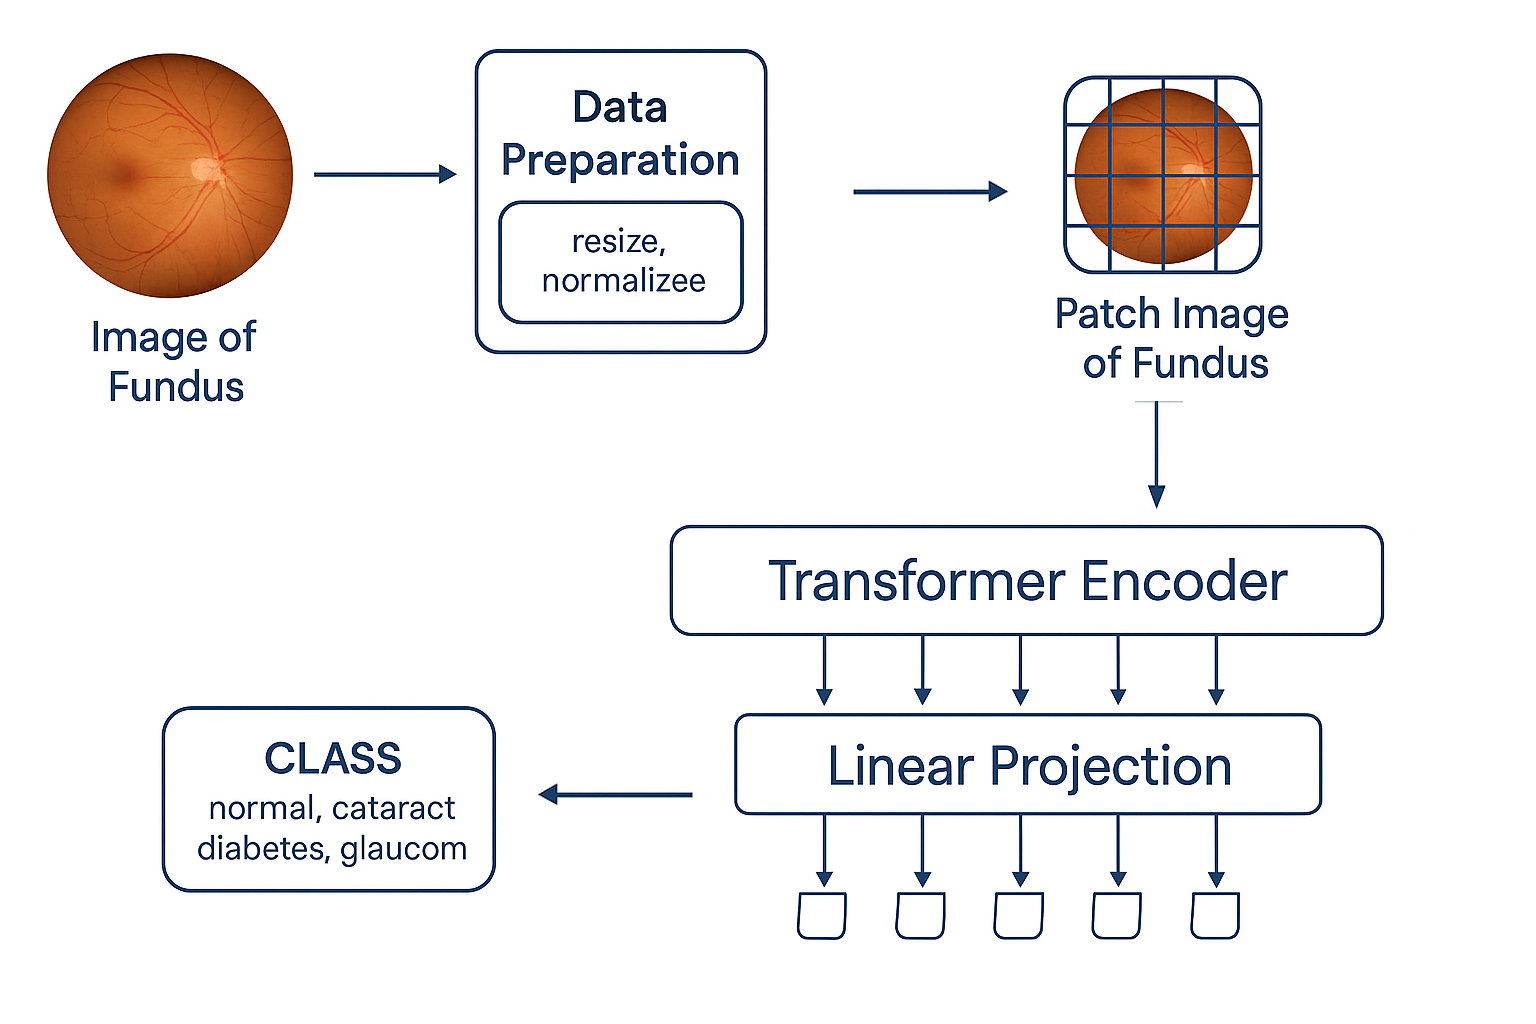
\includegraphics[width=0.4\textwidth]{samples/resources/diagram.png}
  \caption{Image through the model diagram}
  \Description{Diagram of a fundus image going through the ViT model}
\end{figure}


\subsection{Model}
Due to ViTs requiring large amounts of data to be trained on, we will be using a process called transfer learning. Transfer learning is the process of taking the weights of an existing/pre-trained model and then training/fine-tuning from that starting point on a new set of data for faster learning and improved performance. This technique allows smaller datasets to be useful where normally a ViT would only become useful and efficient with datasets like Google’s JFT-300M, which contains over 300 million images \cite{Matsoukas}. Medical pre-trained models are extremely rare to find available publicly due to all the regulations around patient information, therefore we opted to use a generic image model. We chose the “vit\_base\_patch16\_224” PyTorch Image Model. This model was trained on the ImageNet-21k dataset using approximately 14 million images of size 224x224 and used 16x16 size patches during its training \cite{Huggingface}. 

\subsection{Dataset}
We will be using the same retinal image dataset Battalapalli used when training their CNN model [3]. The dataset is called “Eye diseases classification”. it contains 2-dimensional colored retinal images taken from various datasets including  IDRiD, Oculur recognition, HRF \cite{Kaggle}. The is well-balanced with approximately 1,000 images of the following classes: “Normal”, “Cataracts”, “Glaucoma”, and “Diabetic Retinopathy”. The dataset on its own, though relatively small, is expected to be large enough for the ViT model to get performance equal to or greater than Battalapalli’s 80\% accuracy. If need be, data augmentation is considered to increase the amount of training data.

We prepare the data for training by splitting each class into using 70\% of the set for training, 15\% for validation (this will be used during training), and 15\% for testing.  The images from all the classes will be in a single training group and the model will learn those classes at the same time. The images will then be transformed into a size 224x224 pixels to make the images compatible the pre-trained model, the images will be converted to tensors and finally they will be normalized by the mean and standard deviation of the ImageNet dataset to increase the model’s likelihood of good convergence. No data augmentation on the dataset, and the images color scheme was not altered.


\subsection{Training}
For training, we used cross entropy loss, AdamW as the optimizer, CosineAnnealingLR scheduler to fine-tune the learning rate to ensure we could reach the best performance during training. To have our results be comparable to Battalapalli’s training, we opted to train for 7 epochs. We optimized the rest of our hyperparameters to train on a learning rate of 3e-5 using batches of 64. The best results came from freezing half of the layers of the model (block0-block5). Once the hyperparameters were optimized, the model was trained 30 different times with a new randomized training, validation, and testing set for each run to achieve the results.

\subsection{Validation}
For validation, we used the remaining 30\% of the dataset and split it into 2 groups of 15\%. The first group was run during the training to test the model’s performance. The information gathered from the validation allowed us to make decisions about which models were performing best at with what loss. This helped narrow the learning rate and batch sizes early on. 

\subsection{Testing}
For testing we used the last 15\% of the dataset. This set was used to test the model using batches of 64, and metrics were gathered including accuracy, precision, recall, f1-scores across each class. To ensure statistically valid results and as close to true accuracy as possible, the model ran 30 times each with a different training, validation, and test set. Metrics were collected from each run. The pre-trained model was also tested without training to get a baseline of how well the model alone would perform. The accuracy of the pre-trained model ranged from 15\% to 35\% with an average accuracy of 24.55\% across 30 runs (all different test sets).

After training our ViT model’s accuracies ranged from 92\% to 94.98\% accuracy with an average of 93.74\% across 30 runs.
\begin{figure}[h]
  \centering
  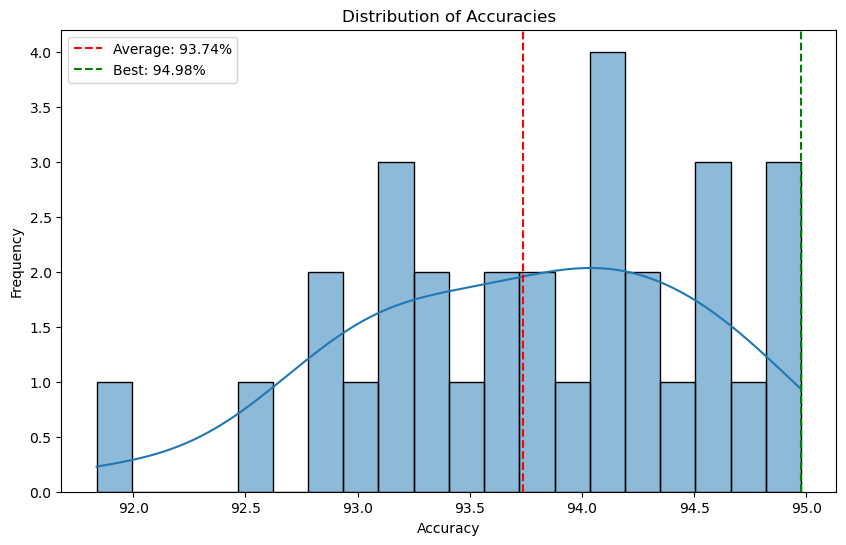
\includegraphics[width=\linewidth]{samples/resources/Accuracy distribution.png}
  \caption{Distribution of accuracies on trained ViT model.}
  \Description{A graph showing all the accuracies across multiple runs of the ViT model}
\end{figure}


\section{Results}
Our ViT model did an excellent job in classifying the retinal images from the dataset. The best performing model reached almost 95\% accuracy on the test set. This alone shows a drastic improvement over the CNNs accuracy we were comparing to. A breakdown of the metrics for our best performing model can be seen in figure X(metrics). The model not only improved overall in the accuracy of classification, but it also drastically improved its accuracy in regard to detecting Glaucoma. The CNN model achieved 46\% precision while our ViT model achieved 93\% precision on the same set trained on the same number of epochs. 


Our macro average precision, recall, and f1-score were almost identical to the weighted averages. This shows that the model was able to generalize with high accuracy. The dataset was well-balanced which would indicate that the macro and weighted average should be very similar, this however was not the case when trained on the CNN architecture where these values differed by 1-5%.

\begin{figure}[h]
  \centering
  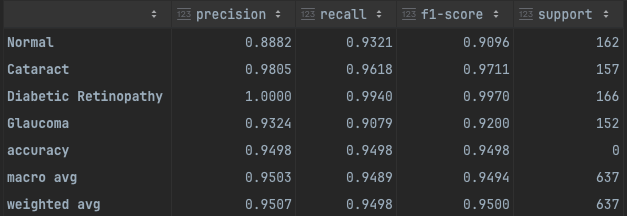
\includegraphics[width=\linewidth]{samples/resources/Metrics.png}
  \caption{ViT Metrics for best model}
  \Description{A table of the metrics of the ViT model for each class tested.}
\end{figure}

A confusion matrix can be seen in figure X2 showing similar results for the accuracy of the model’s predictive ability. With very few false positive and few false negatives, the results show high probability of success for this classification group with a relatively small dataset. Larger datasets and more classes (different retinal disease) are likely to show similar results. 

\begin{figure}[h]
  \centering
  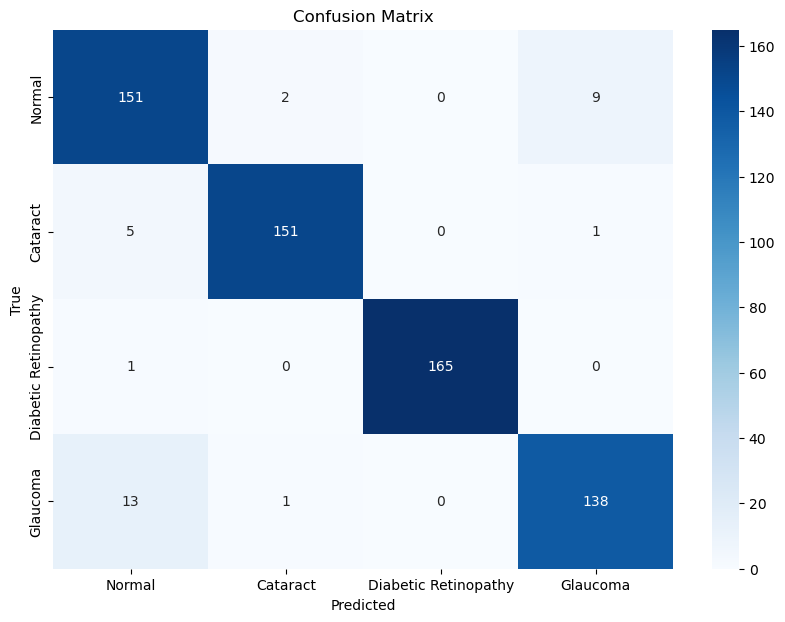
\includegraphics[width=\linewidth]{samples/resources/Confusion Matrix.png}
  \caption{ViT Metrics for best model}
  \Description{A table of the metrics of the ViT model for each class tested.}
\end{figure}

The results expand beyond the metrics of accuracy. As mentioned earlier, vision transformers have an attention mechanism that we can extract to “understand” where the model was giving focus on an image for its prediction. The following figures show a few examples of the image given to the model, the saliency map, which is represented a visual of where the model gives attention to the most on the image, and the saliency map overlay-ed on the original image. This is aspect alone allows the model to be used by ophthalmologists to review a patient’s retinal and have an idea of where to focus or to catch details that would otherwise be hard to spot.

\begin{figure}[]
  \centering
  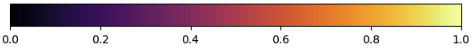
\includegraphics[width=\linewidth]{samples/resources/saliency maps/color map legend.png}
  \caption{Color map legend}
  \Description{A legend of the colors used to denote how much attention the model pays to each pixel}
\end{figure}

\begin{figure}[]
  \centering
  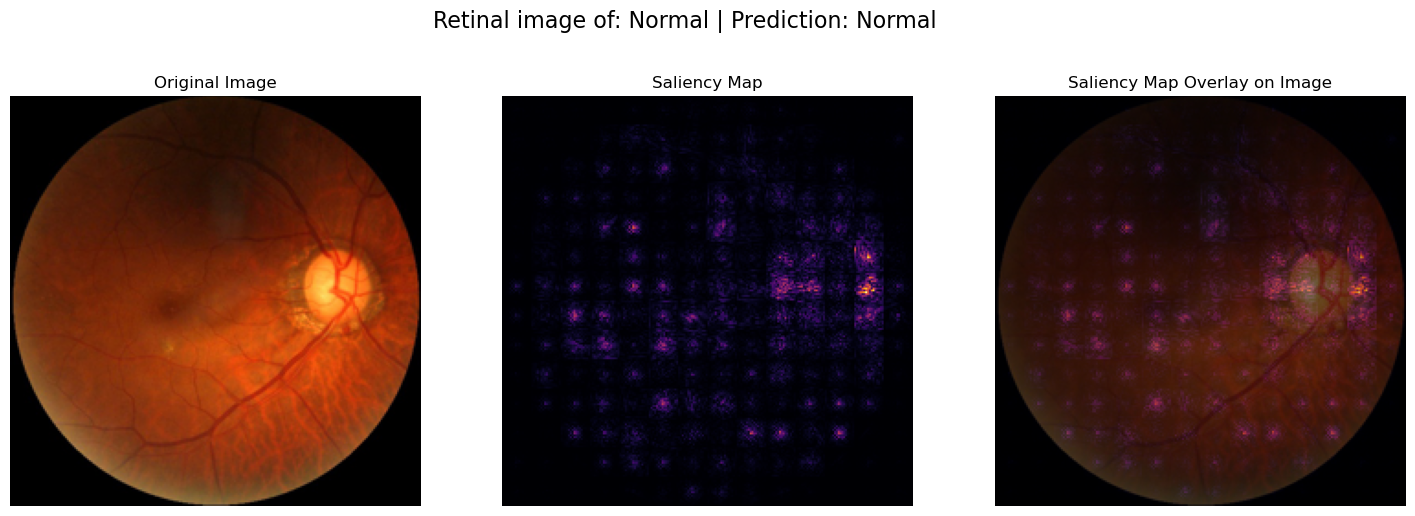
\includegraphics[width=\linewidth]{samples/resources/saliency maps/retinal_normal.png}
  \Description{Retinal images alongside saliency map of areas of attention}
\end{figure}

\begin{figure}[]
  \centering
  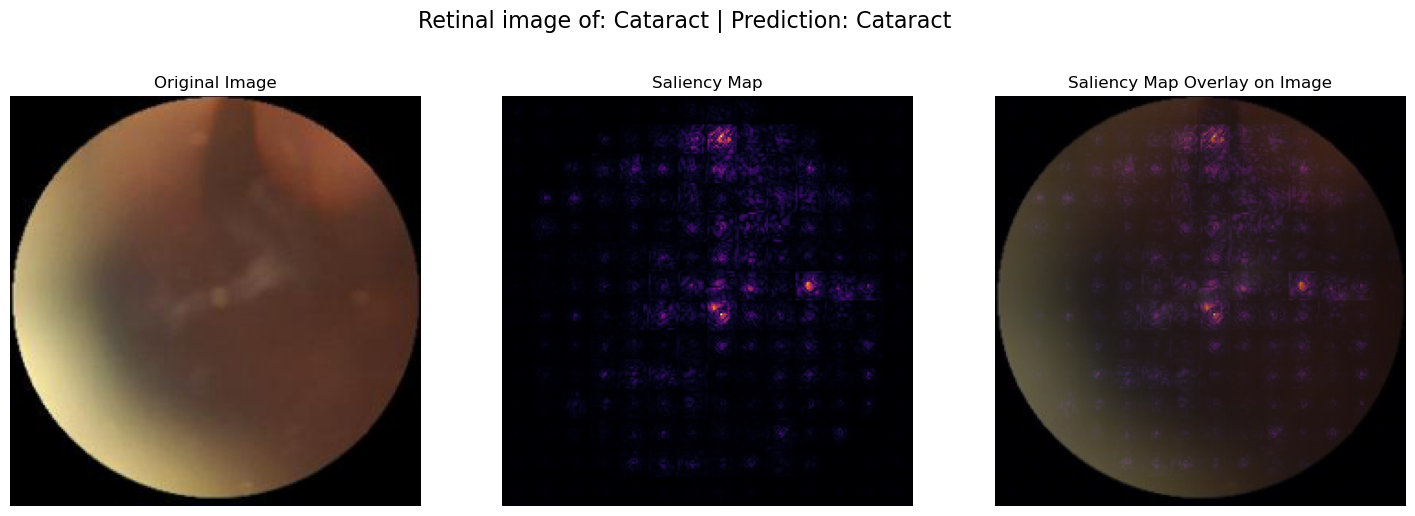
\includegraphics[width=\linewidth]{samples/resources/saliency maps/retinal_cataract.png}
  \Description{Retinal images alongside saliency map of areas of attention}
\end{figure}

\begin{figure}[]
  \centering
  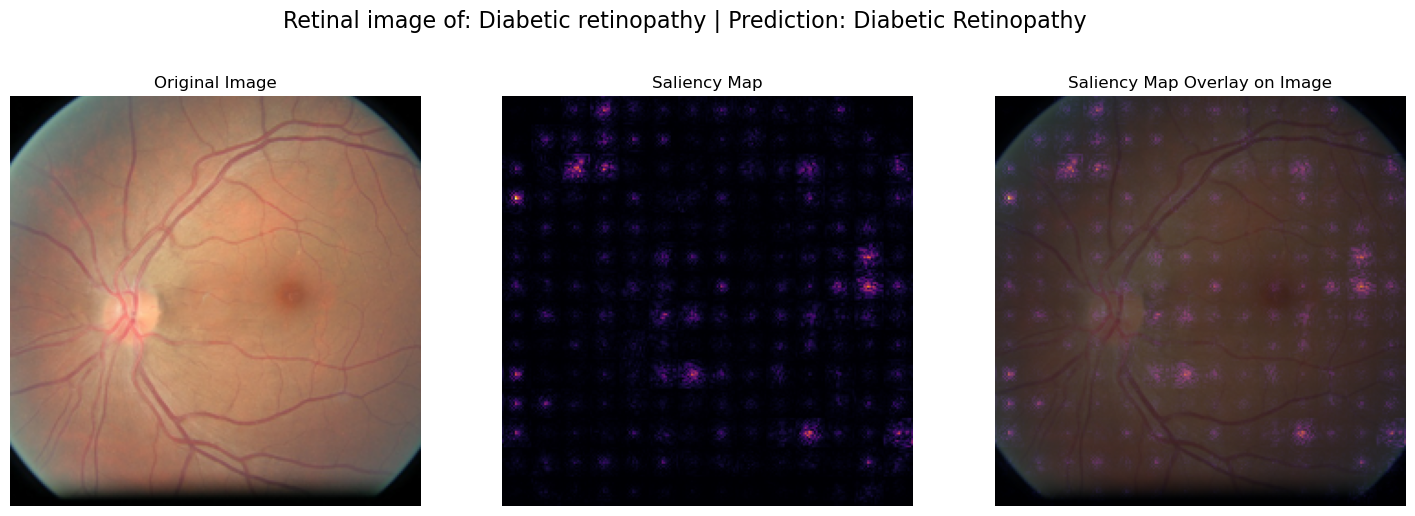
\includegraphics[width=\linewidth]{samples/resources/saliency maps/retinal_diabetic.png}
  \Description{Retinal images alongside saliency map of areas of attention}
\end{figure}

\begin{figure}[]
  \centering
  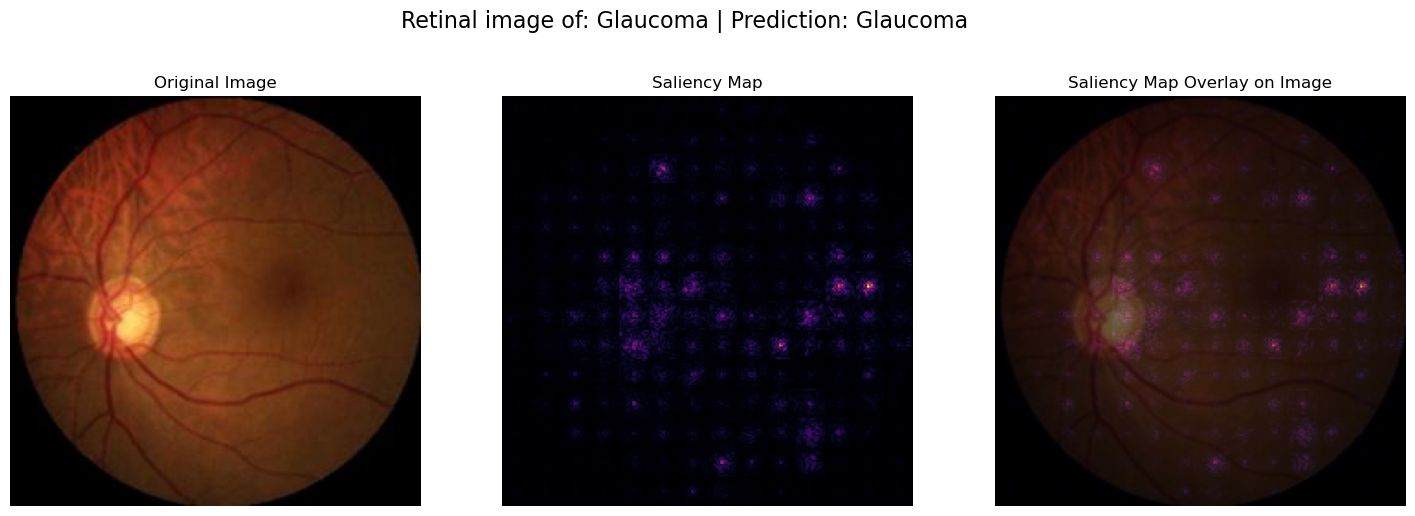
\includegraphics[width=\linewidth]{samples/resources/saliency maps/retinal_glaucoma.png}
  \caption{Retinal Images with Saliency Maps}
  \Description{Retinal images alongside saliency map of areas of attention}
\end{figure}

Included are also some examples were the model predicted incorrectly, these can be used to further train the model. The images as well could in theory be studied more thoroughly as they could be showing early signs of these diseases that the model was able to detect while a human observer may have missed, due to negligible differences or cases where the disease is too early for human observers to detect.

\begin{figure}[]
  \centering
  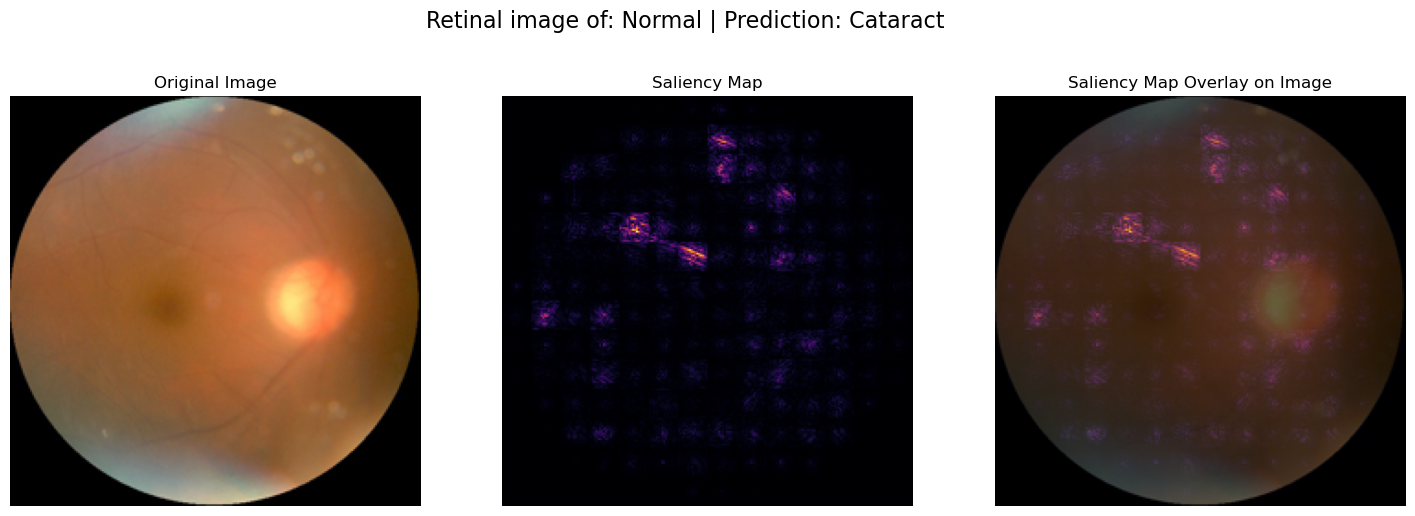
\includegraphics[width=\linewidth]{samples/resources/saliency maps/Normal_as_cataracts.png}
  \Description{Retinal images alongside saliency map of areas of attention}
\end{figure}
\begin{figure}[]
  \centering
  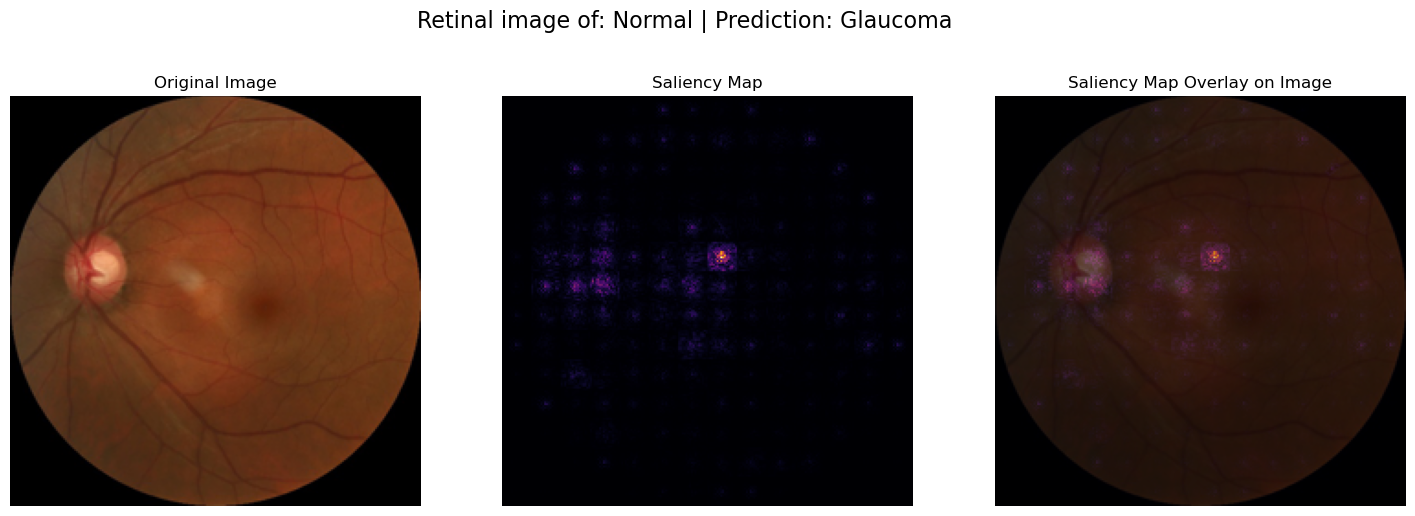
\includegraphics[width=\linewidth]{samples/resources/saliency maps/normal_as_glaucoma_1.png}
  \Description{Retinal images alongside saliency map of areas of attention}
\end{figure}
\begin{figure}[]
  \centering
  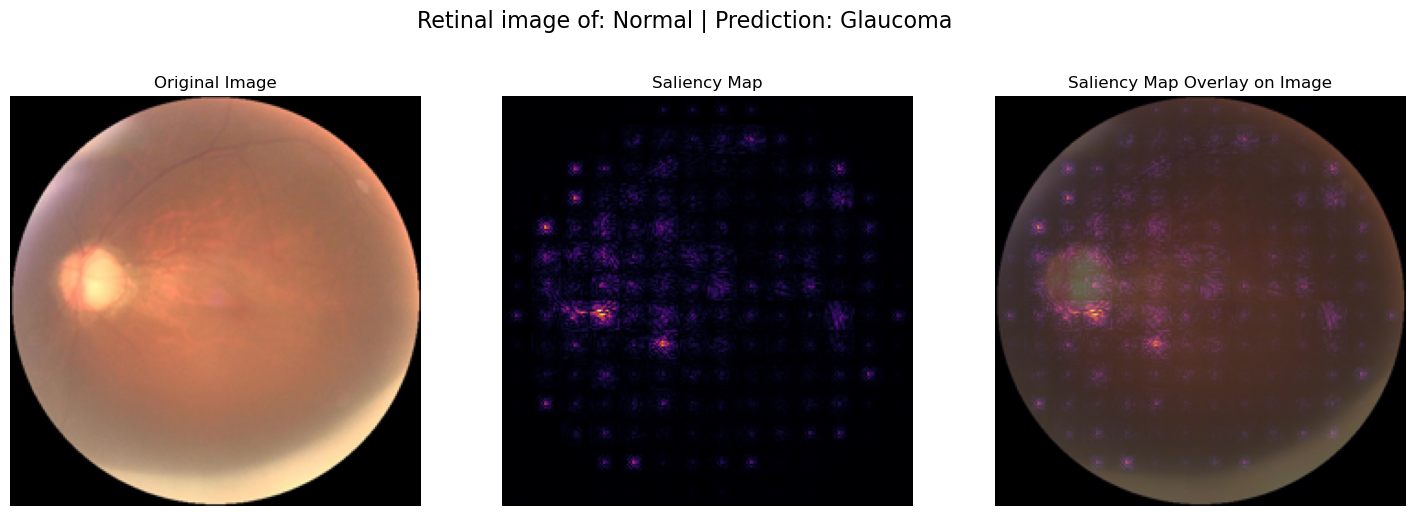
\includegraphics[width=\linewidth]{samples/resources/saliency maps/normal_as_glaucoma_2.png}
  \caption{Retinal Images (incorrect predictions) with Saliency Maps}
  \Description{Retinal images alongside saliency map of areas of attention}
\end{figure}

\section{Conclusion}

The results showed a high level of accuracy and massive improvements over previous retinal classification. The use of visual transformers in image classification in the medical field has a need for more exploration, and improvements on this architecture will only improve the level of detection. Even this experiment can be improved. The data was limited and not data augmentation was used, this could result in higher precision. The disease list was also limited to three diseases and a control group (normal). The model also only tried one pre-trained model and some preliminary training showed that the model was improving past 7 epochs. A deeper dive into where the model's focus through its attention mechanism can be explored for further analysis. One last important improvement to this experiment would be in the use of multimodal models. The classification can further be expanded with an LLM to clarify areas of interest from the saliency maps and why those areas matter. Multimodal training should be considered to improve this model in a way that can be used publicly.

The results from this experiment show that a pre-liminary eye exam conducted by a ViT model can indeed yield highly accurate results. This can reduce cost for patients doing simple exams; while also increasing the amount of patients an ophthalmologists can meet with that require direct help. Less time can be spent doing preliminary work, and more time can be directed at treating the patients who need help. Technology like this also lowers the bar of entry and fear that most people have about having to spend high amounts of money to check their health. This advancement can keep being improved and potentially allow for this exam to be done at home with a phone camera. A few seconds to take a picture of an eye at home, and a patient may have just prevented future blindness due to early detection without any inconvenience.

In the future we hope to expand on this research, with different datasets or with funding from medical institutions. Labeled datasets are massively lacking in the medical field, especially when it comes to public datasets. We hope that we will be able to partner with medical and research facilities to expand the datasets we have, add more diseases and work alongside ophthalmologists to diagnose and find new areas of interest in the retina. 

\section{Acknowledgments}

I'd like to thank the faculty and staff in the Healthcare in Artificial Intelligence class of Spring 2025. A big thak you to Dr. Ying Ding for her lectures knowledge.

%%
%% The next two lines define the bibliography style to be used, and
%% the bibliography file.
\bibliographystyle{ACM-Reference-Format}
\bibliography{References}

\end{document}
\endinput
%%
%% End of file `sample-sigconf-authordraft.tex'.
